\chapter{龙芯新增整型指令}

在标准的 MIPS 指令集中,整点乘法和除法在一个操作中将结果写入两个特殊的寄存
器(HI/LO)中,而它们在 RISC 流水线中很难实现。 为了使用这些结果,往往必须
通过额外的指令把它从 HI/LO 中取出送到通用寄存器中。更麻烦的是,由于流水线问题,
很多 MIPS 处理器对这些指令的使用还有额外的限制。相比之下,这些新增的指令执行
速度更快,没有流水线问题,同时也更容易使用。

\section{新增指令详解}

\subsection{MULT.G (龙芯字乘)}

\begin{instructionblk}
  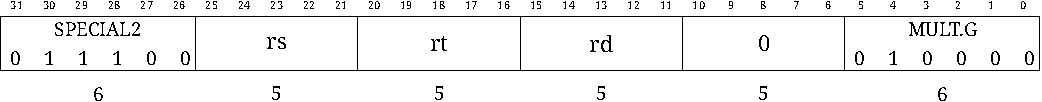
\includegraphics{ins-MULTG} \\
  \instructionbody{MULT.G rd, rs, rt}
  {32 位有符号整数乘。}
  {通用寄存器 rs 中 32 位值乘以通用寄存器 rt 中 32 位值,
  这两个操作数都是有符号数, 产生一个64位结果。 结果的低
  32 位保存在目的寄存器 rd 中。 \fldnewline
  任何情况下都不会产生算术异常。}
  {prod $\leftarrow$ rs[31..0] * rt[31..0]; /* 有符号乘 */ \newline
  rd~~ $\leftarrow$ sign\_extend(prod[31..0]);}
  {无。}
\end{instructionblk}

\subsection{MULTU.G (龙芯无符号字乘)}

\begin{instructionblk}
  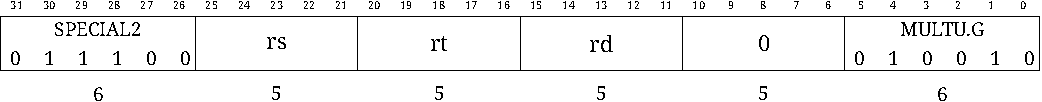
\includegraphics{ins-MULTUG} \\
  \instructionbody
  {MULTU.G rd, rs, rt}
  {32 位无符号整数乘。}
  {通用寄存器rs中32位值乘以通用寄存器rt中32位值,这两个操作数都是无符号数,产
  生一个64位结果。结果的低32位保存在目的寄存器rd中。 \fldnewline
  任何情况下都不会产生算术异常。}
  {prod $\leftarrow$ rs[31..0] * rt[31..0]; /* 无符号乘 */ \newline
  rd~~ $\leftarrow$ sign\_extend(prod[31..0]);}
  {无。}
\end{instructionblk}

\remark{这里有符号扩展?}

\subsection{DMULT.G (龙芯双字乘)}

\begin{instructionblk}
  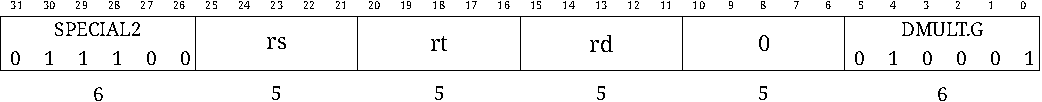
\includegraphics{ins-DMULTG} \\
  \instructionbody
  {DMULT.G rd, rs, rt}
  {64 位有符号整数乘。}
  {通用寄存器rs中64位值乘以通用寄存器rt中64位值,这两个操作数都是有符号数,产
  生一个128位结果。结果的低64位保存在目的寄存器rd中。 \fldnewline
  任何情况下都不会产生算术异常。}
  {prod $\leftarrow$ rs * rt; /* 有符号乘 */ \newline
  rd~~ $\leftarrow$ prod[63..0];}
  {无。}
\end{instructionblk}


\subsection{DMULTU.G (龙芯无符号双字乘)}

\begin{instructionblk}
  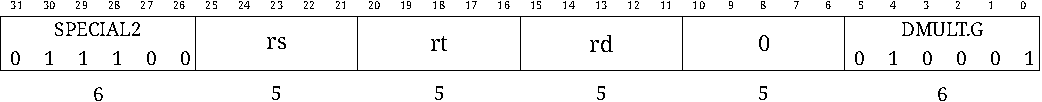
\includegraphics{ins-DMULTG} \\
  \instructionbody
  {DMULTU.G rd, rs, rt}
  {64 位无符号整数乘。}
  {通用寄存器rs中64位值乘以通用寄存器rt中64位值,这两个操作数都是无符号数,产
  生一个128位结果。结果的低64位保存在目的寄存器rd中。\fldnewline
  任何情况下都不会产生算术异常。}
  {prod $\leftarrow$ rs * rt; /* 无符号乘 */ \newline
  rd~~ $\leftarrow$ prod[63..0];}
  {无。}
\end{instructionblk}

\subsection{DIV.G (龙芯字除)}

\begin{instructionblk}
  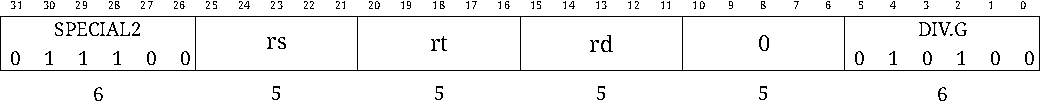
\includegraphics{ins-DIVG} \\
  \instructionbody
  {DIV.G rd, rs, rt}
  {32 位有符号整数除。}
  {通用寄存器rs中32位值除以通用寄存器rt中32位值,这两个操作数都是有符号数。32
  位商保存在目的寄存器rd中。 \fldnewline
  任何情况下都不会产生算术异常。}
  {q~ $\leftarrow$ rs[31..0] div rt[31..0]; /* 有符号除 */ \newline
  rd $\leftarrow$ sign\_extend(q[31..0]);}
  {无。}
\end{instructionblk}

\subsection{DIVU.G (龙芯无符号除)}

\begin{instructionblk}
  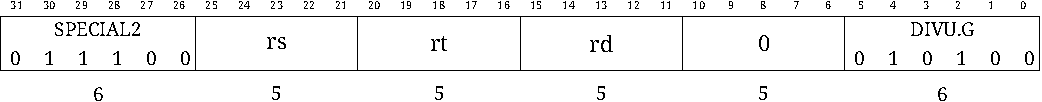
\includegraphics{ins-DIVUG} \\
  \instructionbody
  {DIVU.G rd, rs, rt}
  {32 位无符号整数除。}
  {通用寄存器rs中32位值除以通用寄存器rt中32位值,这两个操作数都是无符号数。32
  位商保存在目的寄存器rd中。 \fldnewline
  任何情况下都不会产生算术异常。}
  {q~ $\leftarrow$ rs[31..0] div rt[31..0]; /* 无符号除 */\newline
  rd $\leftarrow$ sign\_extend(q[31..0]);}
  {无。}
\end{instructionblk}

\subsection{DDIV.G (龙芯双字除)}

\begin{instructionblk}
  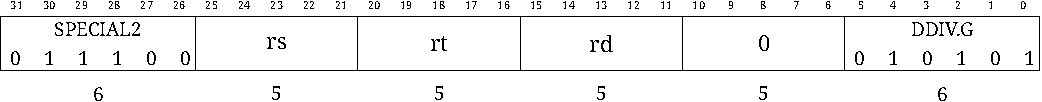
\includegraphics{ins-DDIVG} \\
  \instructionbody
  {DDIV.G rd,rs, rt}
  {64 位有符号整数除。}
  {rd $\leftarrow$ rs / rt \fldnewline
  通用寄存器rs中64位值除以通用寄存器rt中64位值,这两个操作数都是有符号数。64
  位商保存在目的寄存器rd中。 \fldnewline
  任何情况下都不会产生算术异常。}
  {rd $\leftarrow$ rs div rt; /* 有符号除 */}
  {无。}
\end{instructionblk}

\subsection{DDIVU.G (龙芯无符号双字除)}

\begin{instructionblk}
  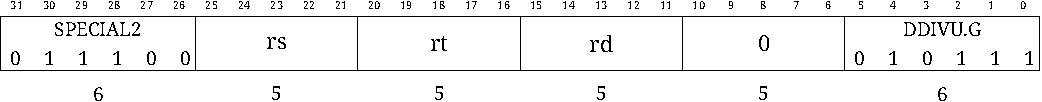
\includegraphics{ins-DDIVUG} \\
  \instructionbody
  {DDIVU.G rd, rs, rt}
  {64 位无符号整数除。}
  {通用寄存器rs中64位值除以通用寄存器rt中64位值,这两个操作数都是无符号数。64
  位商保存在目的寄存器rd中。 \fldnewline
  任何情况下都不会产生算术异常。}
  {rd $\leftarrow$ rs div rt; /* 无符号除 */}
  {无。}
\end{instructionblk}

\subsection{MOD.G (龙芯字求模)}

\begin{instructionblk}
  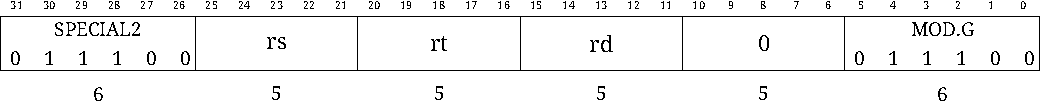
\includegraphics{ins-MODG} \\
  \instructionbody
  {MOD.G rd, rs, rt}
  {32 位有符号整数求模。}
  {通用寄存器rs中32位值除以通用寄存器rt中32位值,这两个操作数都是有符号数。32
  位剩余数保存在目的寄存器rd中。 \fldnewline
  任何情况下都不会产生算术异常。}
  {q~ $\leftarrow$ rs[31..0] mod rt[31..0]; /* 有符号求模 */ \newline
  rd $\leftarrow$ sign\_extend(q[31..0]);}
  {无。}
\end{instructionblk}

\subsection{MODU.G (龙芯无符号字求模)}

\begin{instructionblk}
  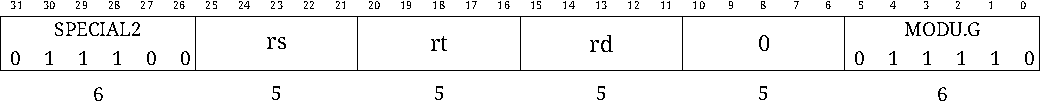
\includegraphics{ins-MODUG} \\
  \instructionbody
  {MODU.G rd, rs, rt}
  {32 位无符号整数求模。}
  {通用寄存器rs中32位值除以通用寄存器rt中32位值,这两个操作数都是无符号数。32
  位剩余数保存在目的寄存器rd中。 \fldnewline
  任何情况下都不会产生算术异常。}
  {q~ $\leftarrow$ rs[31..0] mod rt[31..0]; /* 无符号求模 */ \newline
  rd $\leftarrow$ sign\_extend(q[31..0]);}
  {无。}
\end{instructionblk}

\subsection{DMOD.G (龙芯双字求模)}

\begin{instructionblk}
  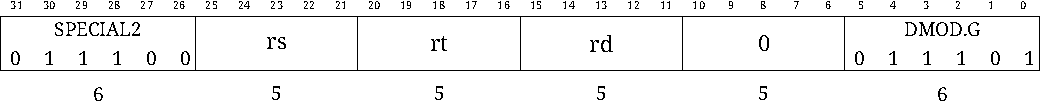
\includegraphics{ins-DMODG} \\
  \instructionbody
  {DMOD.G rd, rs, rt}
  {64 位有符号整数求模。}
  {通用寄存器rs中64位值除以通用寄存器rt中64位值,这两个操作数都是有符号数。64
  位剩余数保存在目的寄存器rd中。 \fldnewline
  任何情况下都不会产生算术异常。}
  {rd $\leftarrow$ rs mod rt; /* 有符号求模 */}
  {无。}
\end{instructionblk}

\subsection{DMODU.G (龙芯无符号双字求模)}

\begin{instructionblk}
  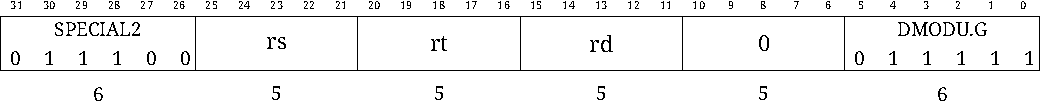
\includegraphics{ins-DMODUG} \\
  \instructionbody
  {DMODU.G rd, rs, rt}
  {64 位无符号整数求模。}
  {通用寄存器rs中64位值除以通用寄存器rt中64位值,这两个操作数都是无符号数。64
  位剩余数保存在目的寄存器rd中。 \fldnewline
  任何情况下都不会产生算术异常。}
  {rd $\leftarrow$ rs mod rt; /* 无符号求模 */}
  {无。}
\end{instructionblk}

